\documentclass[11pt]{article}
% ---- fill these two in before the final build (see ZENODO_UPLOAD.md) ----
\newcommand{\repourl}{https://github.com/wasifhaq434701-png/Cortex-mem}
\newcommand{\reportdoi}{10.5281/zenodo.23376016}  % e.g. 10.5281/zenodo.1234567 (Zenodo "reserve DOI"); leave empty to omit
% ---------------------------------------------------------------------------
\usepackage[margin=1in]{geometry}
\usepackage{times}
\usepackage[T1]{fontenc}
\renewcommand{\ttdefault}{lmtt}  % newtx typewriter font is not in BasicTeX
\usepackage{microtype}
\usepackage{graphicx}
\usepackage{booktabs}
\usepackage{multirow}
\usepackage{amsmath}
\usepackage{xcolor}
\usepackage[font=small,labelfont=bf]{caption}
\usepackage[numbers,sort&compress]{natbib}
\usepackage[colorlinks=true,linkcolor=black,citecolor=black,urlcolor={rgb:red,0.16;green,0.47;blue,0.84}]{hyperref}

\title{\bfseries Parameter-Level Conditional Computation\\Does Not Buy Quality on Phones:\\Three Negative Results for On-Device LLMs}
\author{Mohammed Wasif Ul Haq\\[2pt]
\small Independent researcher \quad \texttt{wasif.haq434701@gmail.com}}
\date{Technical report v1 --- October 2026}

\begin{document}
\maketitle
\ifx\reportdoi\empty\else\begin{center}\small DOI: \href{https://doi.org/\reportdoi}{\reportdoi}\end{center}\fi

\begin{abstract}
\noindent Token generation on phones is bound by memory bandwidth, so the quality a phone can serve is set
by how many parameter bytes it can afford to read per token. A tempting way around this limit is
\emph{conditional computation at the parameter level}: use a cheap signal about the request (its task)
to keep only the parameters that request needs in RAM, or to load a small task-specific module. We test
this idea three ways on an Apple M4 Max, each against a fair dense or shared baseline. (1) Expert usage in
Qwen3-30B-A3B is genuinely task-local (a task-predicted resident set of 32 of 128 experts per layer serves
64\% of decode-time expert reads, versus 49\% for a task-agnostic set), but the remaining misses still
cost about 210\,MB of flash reads per token at a 7\,GB budget. (2) Routing only among resident experts
removes those reads but collapses generation quality long before phone budgets (GSM8K 94\%\,$\to$\,10\%
at 7\,GB of resident weights), while a dense 8B model in 4.6\,GB scores 89\%; seven training-free rescue
variants do not help. (3) A dense 4B core with per-task LoRA modules chosen per request (by oracle or by an
embedding router) is within noise of a single shared multi-task LoRA on all four evaluations, at equal
per-request cost and at equal storage. Along the way we find that fine-tuning on dataset reference
answers damages a strong instruction-tuned core on every task, while self-distilled data does not, and
that sentence-embedding routing misroutes 27\% of DROP questions. Per-request selection appears
necessary only for state that a shared model cannot hold, such as an individual user's data. All code,
data, per-item scores and generations are released.
\end{abstract}

\section{Introduction}
During autoregressive decoding, each generated token reads every active weight once, so throughput on a
bandwidth-bound device is roughly
\begin{equation}
\text{tokens/s} \approx \frac{\text{memory bandwidth}}{\text{active bytes per token}} .
\end{equation}
Phones have small RAM and modest bandwidth compared with servers, which caps both the size of model that
fits and the speed at which it runs. Mixture-of-experts (MoE) models decouple total from active
parameters, and adapters (LoRA~\cite{hu2021lora}) add task capacity for a few megabytes. Both suggest
the same design: \emph{decide once per request which parameters matter, and keep only those resident.}
A request-level decision is attractive on device because it yields a fixed parameter set, hence a
static compute graph, for the whole request, and loads from flash only at request boundaries.

We ask whether this design buys quality inside a fixed RAM budget, and answer it with three experiments
of increasing generosity to the idea:
\begin{itemize}\raggedright
\item \textbf{Exp.~1} measures whether MoE expert usage is predictable from the task at all (it is).
\item \textbf{Exp.~2} keeps only task-predicted experts resident and forbids routing to the rest, so no
flash reads occur during decoding; it fails, and training-free repairs do not help.
\item \textbf{Exp.~3} gives the idea its best shot: a dense core plus small \emph{trained} task modules,
compared against one shared module of equal per-request cost and of equal storage; the task modules
never win beyond noise.
\end{itemize}
All three are negative results. We report them in full because each rules out a design that is natural
to try, and because together they point to where request-level selection \emph{is} necessary
(Section~\ref{sec:discussion}).

\section{Setup}
All experiments ran on a MacBook Pro (M4 Max, 36\,GB unified memory, macOS 27) with MLX 0.31.2 and
\texttt{mlx-lm} 0.31.3, using 4-bit community conversions of Qwen3 models~\cite{qwen3} in non-thinking
mode with greedy decoding. Benchmarks: GSM8K~\cite{cobbe2021gsm8k} (exact numeric answer),
HumanEval~\cite{chen2021humaneval}, MBPP~\cite{austin2021mbpp} (training only), and
DROP~\cite{dua2019drop}. Every script, the per-item scores behind each number, and all raw generations
are in the repository (\url{\repourl}).

\section{Experiment 1: is expert usage task-local?}
\paragraph{Method.} Qwen3-30B-A3B has 48 MoE layers with 128 experts each and routes every token to 8
experts per layer; the 4-bit model is 17.2\,GB, of which 0.9\,GB is non-expert weights. We generated 128
greedy tokens for 25 hand-written prompts (5 each for code, math, personal notes, chat and writing) and
recorded every expert selection. For a budget of $K$ resident experts per layer we measure the decode-time
\emph{hit rate}: the fraction of expert selections served by the resident set. Resident sets are chosen,
leave-one-out, as the request's own top-$K$ (oracle, an upper bound), the top-$K$ of the other requests of
the same task (\emph{task}, what a request-level predictor could do), or the top-$K$ of all other requests
(\emph{global}, static pruning).

\begin{table}[h]
\centering\small
\caption{Decode-time hit rate (\%) of the resident expert set, all 25 prompts. The last column converts
task-predicted misses into flash reads per generated token.}
\label{tab:exp1}
\begin{tabular}{rrrrrrr}
\toprule
$K$/128 & resident GB & oracle & task & global & random & misses (MB/token) \\
\midrule
16 & 2.9 & 60.3 & 41.7 & 29.3 & 12.5 & 594 \\
32 & 4.9 & 81.8 & 64.2 & 49.1 & 25.0 & 365 \\
48 & 7.0 & 92.5 & 79.4 & 65.4 & 37.5 & 210 \\
64 & 9.0 & 97.5 & 88.8 & 77.9 & 50.0 & 114 \\
\bottomrule
\end{tabular}
\end{table}

\paragraph{Result.} Locality is real (Table~\ref{tab:exp1}): at $K{=}32$ the task-predicted set serves 64\%
of reads against 49\% for a task-agnostic set and 25\% at random. The task signal matters most for code
(56\% vs.\ 32\%) and math (59\% vs.\ 33\%); for chat and personal notes the task and global sets are close
(62 vs.\ 59, 64 vs.\ 57), consistent with shared ``general language'' experts. Prefill on these short
prompts touches 50--65\% of all experts. The problem is the misses: even at $K{=}48$, about 79 expert
loads per token remain, roughly 210\,MB of reads per generated token. At 20 tokens/s that is
${\sim}4$\,GB/s of random flash reads, far beyond what flash-offloading systems
budget~\cite{alizadeh2023flash,xue2024powerinfer2}. Loading misses on demand is not viable, which motivates
Experiment~2.

\section{Experiment 2: route only among resident experts}
\paragraph{Method.} We hard-mask the router so each token picks its top-8 experts \emph{only} among the
resident set (``reroute''), which eliminates flash reads during decoding. Resident sets are calibrated on
the full model's routing over GSM8K train[:50] and HumanEval[:40], and evaluated on GSM8K test[:100]
(accuracy) and on teacher-forced NLL per token of the canonical HumanEval[40:] solutions (124 problems).
We also tried seven training-free rescue variants: larger budgets; ``drop'' (keep the router's original
top-8, zero non-resident picks and renormalise); and adaptive per-layer budgets that give more slots to
layers whose routing is more spread out, at equal total size.

\begin{figure}[t]
\centering
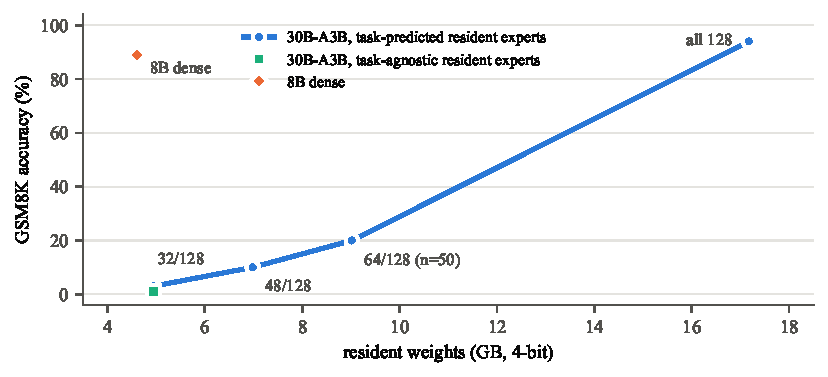
\includegraphics[width=0.88\linewidth]{fig_exp2.pdf}
\caption{GSM8K accuracy against resident weight size. Masking Qwen3-30B-A3B's router to a
task-predicted resident set collapses quality long before phone-scale budgets; a dense 8B model in 4.6\,GB
scores 89\%. The 64/128 point uses the first 50 test questions.}
\label{fig:exp2}
\end{figure}

\begin{table}[h]
\centering\small
\caption{Constrained routing on Qwen3-30B-A3B. ``task'' / ``global'': resident set calibrated per task /
once for all tasks. Rows below the rule use GSM8K test[:50].}
\label{tab:exp2}
\begin{tabular}{lrrr}
\toprule
configuration & resident GB & GSM8K (\%) & code NLL/token \\
\midrule
Qwen3-8B dense & 4.6 & 89 & 0.671 \\
Qwen3-30B-A3B, all experts & 17.2 & 94 & 0.676 \\
task set, $K{=}48$, reroute & 7.0 & 10 & 0.788 \\
task set, $K{=}32$, reroute & 4.9 & 3 & 0.814 \\
global set, $K{=}32$, reroute & 4.9 & 1 & 1.354 \\
\midrule
task set, $K{=}64$, reroute & 9.0 & 20 & 0.739 \\
task set, $K{=}64$, drop & 9.0 & 8 & 0.795 \\
task set, $K{=}48$, drop & 7.0 & 2 & 1.220 \\
task set, $K{=}32$, drop & 4.9 & 0 & 1.375 \\
task set, adaptive 48/layer avg., drop & 7.0 & 2 & 1.426 \\
task set, adaptive 32/layer avg., reroute & 4.9 & 4 & 2.030 \\
task set, adaptive 32/layer avg., drop & 4.9 & 2 & 1.968 \\
\bottomrule
\end{tabular}
\end{table}

\paragraph{Result.} Quality collapses (Figure~\ref{fig:exp2}, Table~\ref{tab:exp2}). Keeping half the
experts already drops GSM8K from 94\% to 20\%; at 7\,GB it is 10\%, while the dense 8B model scores 89\% in
4.6\,GB. We inspected the outputs: at $K{=}64$ generations stay coherent but wordier, and at $K{=}48$ they
fall into repetition loops. Two observations matter beyond this model. First, teacher-forced NLL hides the
cliff (0.676\,$\to$\,0.788 at $K{=}48$) while generation fails: small per-layer rerouting errors compound
over 48 layers and over generated tokens. Second, task-calibrated sets beat the task-agnostic set at equal
size (NLL 0.814 vs.\ 1.354), so the task signal is informative; it is simply not enough to replace
training. ``Drop'' is worse than ``reroute'', and adaptive per-layer budgets hurt, suggesting that layers
cannot be pruned independently. Post-hoc expert residency does not work without training; MoE models
built for phones are instead trained for the device from the start~\cite{mobilemoe}, and task-level
routing has succeeded when it is trained in~\cite{kudugunta2021beyond}.

\section{Experiment 3: dense core plus per-task modules}
\label{sec:exp3}
Experiment~2 shows that parameters cannot be removed after training. The trained version of the same idea
is a dense core plus small task modules, trained with the sparsity they run with, selected once per
request and loaded from flash in megabytes rather than per token. This is the setting of LoRA libraries
and routers such as LoraHub~\cite{huang2023lorahub}, MoLE~\cite{wu2024mole}, X-LoRA~\cite{buehler2024xlora}
and Arrow~\cite{ostapenko2024arrow}. The question is whether choosing a module per request beats simply
training one shared module.

\paragraph{Design.} Core: Qwen3-4B (4-bit). Three tasks, each with training data disjoint from its evaluation:
\emph{math} (GSM8K train $\to$ GSM8K test[:250], accuracy); \emph{code} (all 974 MBPP problems $\to$
HumanEval, 164 problems, pass@1 by executing the official tests in an isolated subprocess); and
\emph{notes}, an equal mix of DROP training questions and a synthetic personal-notes benchmark we
release. Its items are short notes mixing bills, birthdays, medication and warranties, with questions
whose answers must be computed (sums, date differences, expiry years), and the other facts act as
distractors. Train and test use disjoint name, item and medication pools and disjoint phrasings of every
fact and question, so test gains require transfer rather than template memorisation. Notes is evaluated on
200 held-out synthetic items (exact match) and 300 DROP validation questions (EM/F1, number and span
answers), always reported separately.

Adapters: LoRA on every linear layer of all 36 blocks, rank 8 (66\,MB as saved), batch 4, prompt-masked
loss, maximum length 1024. Baselines: no adapter; \emph{multi-r8}, one LoRA on the union of the three
training sets with the same rank (equal per-request cost); and \emph{multi-r24}, rank 24 (equal storage to
all three task adapters). The shared adapters train for three times as many steps, so they see as many
examples as the three task adapters combined. Because \texttt{mlx-lm}'s LoRA scale multiplies the update
directly, we keep scale$\times$rank constant (scale 20 at rank 8, $20\cdot 8/24$ at rank 24); rank 24 at
scale 20 diverged within 40 steps. Every adapter is evaluated on every set, so the \emph{oracle}
(each item scored under its own task's adapter) and \emph{routed} conditions follow from the same
per-item scores without reloading models. The router is Cortex-style~\cite{ulhaq2026cortex}: it embeds the
request with all-MiniLM-L6-v2~\cite{wang2020minilm} and picks the task whose centroid of 300 training
prompts is nearest by cosine similarity.

\paragraph{Round 1: reference answers damage the core.} We first trained on dataset reference answers
(GSM8K solutions, MBPP code, synthetic rationales, DROP gold answers; 600 steps, learning rate
$10^{-4}$). Every adapter got worse on its own task except notes (Table~\ref{tab:exp3r1}). Inspecting the
outputs shows why: GSM8K references and MBPP solutions are terser and sloppier than the 4B's own answers,
so the adapters learned a worse style. They also collapsed off-task: the code adapter answers GSM8K
questions with code (6\%), and the math adapter writes prose instead of code (HumanEval 3.7\%). This
matches the distribution-gap explanation of fine-tuning damage in~\cite{yang2024sdft}.

\begin{table}[h]
\centering\small
\caption{Round 1 (reference-answer fine-tuning). Rows are adapters, columns evaluation sets (\%).
Diagonal entries in bold.}
\label{tab:exp3r1}
\begin{tabular}{lrrrr}
\toprule
adapter & GSM8K & HumanEval & notes EM & DROP EM \\
\midrule
none (base) & 88.0 & 77.4 & 57.5 & 60.7 \\
math & \textbf{63.2} & 3.7 & 37.5 & 36.0 \\
code & 6.0 & \textbf{32.3} & 4.5 & 6.7 \\
notes & 15.6 & 0.0 & \textbf{74.0} & \textbf{40.7} \\
multi-r8 & 57.2 & 37.2 & 74.5 & 48.7 \\
\bottomrule
\end{tabular}
\end{table}

\paragraph{Round 2: self-distilled data (the reported run).} Following~\cite{yang2024sdft}, we regenerated
every training set from the base model's own greedy answers and kept only correct ones: matching GSM8K
answer (1809 of 2050 kept), passing all MBPP tests (618 of 974), and exact match on notes and DROP (1048 of
2050); examples longer than 1024 tokens were dropped. We trained 300 steps per task adapter (900 for the
shared adapters) at learning rate $2\cdot10^{-5}$. Uncertainty is a 95\% paired bootstrap over evaluation
items (10{,}000 resamples). The base model's DROP EM differs from round~1 by 0.6 points (61.3 vs.\ 60.7)
because the two runs batched prompts differently, which changes a few numerically borderline greedy
generations.

\begin{table}[h]
\centering\small
\caption{Round 2 (self-distilled fine-tuning), \% on each evaluation set ($n$ = 250, 164, 200, 300).}
\label{tab:exp3r2}
\begin{tabular}{lrrrrr}
\toprule
configuration & GSM8K & HumanEval & notes EM & DROP EM & DROP F1 \\
\midrule
no adapter & 88.0 & 77.4 & 57.5 & 61.3 & 69.1 \\
math adapter & 88.0 & 79.3 & 66.0 & 65.0 & 70.3 \\
code adapter & 88.8 & 76.2 & 58.0 & 60.0 & 67.2 \\
notes adapter & 88.8 & 78.0 & 69.0 & 66.3 & 72.1 \\
\midrule
oracle task adapter & 88.0 & 76.2 & 69.0 & 66.3 & 72.1 \\
routed task adapter & 88.0 & 76.2 & 69.0 & 64.0 & 69.6 \\
shared multi-r8 (equal cost) & 86.4 & 80.5 & 67.0 & 66.0 & 71.6 \\
shared multi-r24 (equal storage) & 88.4 & 78.0 & 67.5 & 64.3 & 70.7 \\
\bottomrule
\end{tabular}
\end{table}

\begin{figure}[t]
\centering
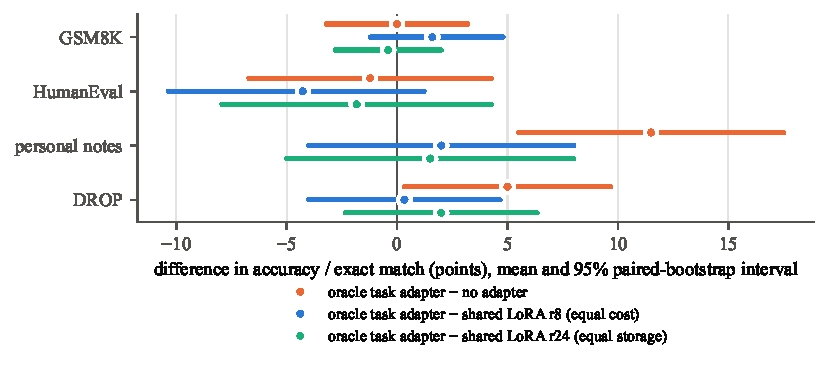
\includegraphics[width=0.88\linewidth]{fig_exp3.pdf}
\caption{Paired differences with 95\% bootstrap intervals. Task adapters beat the bare core only on
personal notes and DROP, and are indistinguishable from a single shared LoRA everywhere.}
\label{fig:exp3}
\end{figure}

\paragraph{Result.} Self-distillation removes the damage: no adapter is below the base on any set
(Table~\ref{tab:exp3r2}). The oracle task adapters improve on the bare core only where it had headroom:
notes $+11.5$ points [5.5, 17.5] and DROP $+5.0$ [0.3, 9.7]; math and code are unchanged, as training on
answers the model already gets right teaches it little. The central comparison is null
(Figure~\ref{fig:exp3}). Oracle task adapters versus the equal-cost shared adapter differ by $+1.6$,
$-4.3$, $+2.0$ and $+0.3$ points, and versus the equal-storage shared adapter by $-0.4$, $-1.8$, $+1.5$ and
$+2.0$; every interval contains zero. Much of the notes gain is not even task-specific: the \emph{math}
adapter alone improves notes by 8.5 points, plausibly through more reliable answer formatting. The router
is perfect on GSM8K and notes and 99.4\% on HumanEval, but routes only 73\% of DROP questions to the notes
adapter (66\% in round~1), because number-heavy passages look like math to a sentence embedding. This
costs 2.3 points of DROP EM relative to the oracle.

\section{Discussion}
\label{sec:discussion}
\paragraph{What the three results rule out.} With a cheap request-level signal, it is possible to predict
which parameters a request uses (Exp.~1). But removing the rest after training destroys generation
(Exp.~2), and training separate modules to select among buys nothing over training one shared module
(Exp.~3). In Exp.~3 the shared adapter had no interference to avoid: once the training data matched the
core's own distribution, no adapter hurt any other task. A conditional design only pays when what is
selected cannot be shared.

\paragraph{Where selection is necessary.} One class of state cannot be shared by construction: an
individual user's data. A single model cannot contain every user's private history, so per-user state
must be stored separately and selected per request. This argues for spending the device's
conditional-computation budget on a user's memory rather than on model parameters: select which
user-specific context or state to bring into a fixed RAM budget for a request, as context selection does
for local retrieval~\cite{ulhaq2026cortex}. We are evaluating this on long-term memory benchmarks such as
LongMemEval~\cite{wu2024longmemeval} and LoCoMo~\cite{maharana2024locomo}, and measuring on a phone.

\paragraph{Limitations.} All results use one core model per experiment, a single seed, and a laptop rather
than a phone; on-device speed, energy and thermal behaviour are not measured here. Experiment~1 uses 25
hand-written prompts. Experiment~3 has three tasks, two of which the core already handles well; tasks
where a 4B core is weak may show larger adapter gains, and with more tasks a single rank-8 adapter may
saturate where a library would not. The personal-notes benchmark is synthetic and was built by us.
Mixed-task requests, the expected weak point of request-level routing, were not tested; given the null
result on single-task requests we do not expect them to reverse the conclusion.

\section{Reproducibility}
Code, training data for both rounds, per-item scores, every generation and every training log are in the
repository, \url{\repourl}:
\begin{itemize}\raggedright
\item Exp.~1: \texttt{experiments/expert\_locality.py}
\item Exp.~2: \texttt{experiments/routing\_quality.py}
\item Exp.~3: \texttt{experiments/task\_adapters.py} (commands \texttt{distill}, \texttt{train},
\texttt{eval}, \texttt{report}) and \texttt{experiments/notes\_synth.py}
\end{itemize}
Experiment~3 takes about 11 hours on an M4 Max; \texttt{report} recomputes every Exp.~3 number and
interval from the committed per-item scores without a GPU. Adapter weights (about 700\,MB) are available
from the author.

\paragraph{Acknowledgements.} The experiment code, analysis and drafting of this report were done with the
assistance of Claude (Anthropic), an AI model. The author directed the research and is responsible for
its content.

\small
\begin{thebibliography}{99}
\bibitem{alizadeh2023flash} K.~Alizadeh, I.~Mirzadeh, D.~Belenko, et al. LLM in a flash: Efficient large language model inference with limited memory. arXiv:2312.11514, 2023.
\bibitem{austin2021mbpp} J.~Austin, A.~Odena, M.~Nye, et al. Program synthesis with large language models. arXiv:2108.07732, 2021.
\bibitem{buehler2024xlora} E.~L.~Buehler and M.~J.~Buehler. X-LoRA: Mixture of low-rank adapter experts, a flexible framework for large language models with applications in protein mechanics and molecular design. \emph{APL Machine Learning}, 2024. arXiv:2402.07148.
\bibitem{chen2021humaneval} M.~Chen, J.~Tworek, H.~Jun, et al. Evaluating large language models trained on code. arXiv:2107.03374, 2021.
\bibitem{cobbe2021gsm8k} K.~Cobbe, V.~Kosaraju, M.~Bavarian, et al. Training verifiers to solve math word problems. arXiv:2110.14168, 2021.
\bibitem{dua2019drop} D.~Dua, Y.~Wang, P.~Dasigi, G.~Stanovsky, S.~Singh, and M.~Gardner. DROP: A reading comprehension benchmark requiring discrete reasoning over paragraphs. In \emph{NAACL}, 2019. arXiv:1903.00161.
\bibitem{hu2021lora} E.~J.~Hu, Y.~Shen, P.~Wallis, et al. LoRA: Low-rank adaptation of large language models. In \emph{ICLR}, 2022. arXiv:2106.09685.
\bibitem{huang2023lorahub} C.~Huang, Q.~Liu, B.~Y.~Lin, T.~Pang, C.~Du, and M.~Lin. LoraHub: Efficient cross-task generalization via dynamic LoRA composition. In \emph{COLM}, 2024. arXiv:2307.13269.
\bibitem{kudugunta2021beyond} S.~Kudugunta, Y.~Huang, A.~Bapna, M.~Krikun, D.~Lepikhin, M.-T.~Luong, and O.~Firat. Beyond distillation: Task-level mixture-of-experts for efficient inference. In \emph{Findings of EMNLP}, 2021. arXiv:2110.03742.
\bibitem{maharana2024locomo} A.~Maharana, D.-H.~Lee, S.~Tulyakov, M.~Bansal, F.~Barbieri, and Y.~Fang. Evaluating very long-term conversational memory of LLM agents. In \emph{ACL}, 2024. arXiv:2402.17753.
\bibitem{mobilemoe} Y.~Chen, H.~Huang, E.~Chang, et al. MobileMoE: Scaling on-device mixture of experts. arXiv:2605.27358, 2026.
\bibitem{ostapenko2024arrow} O.~Ostapenko, Z.~Su, E.~M.~Ponti, et al. Towards modular LLMs by building and reusing a library of LoRAs. In \emph{ICML}, 2024. arXiv:2405.11157.
\bibitem{qwen3} Qwen Team. Qwen3 technical report. arXiv:2505.09388, 2025.
\bibitem{ulhaq2026cortex} M.~W.~Ul~Haq. What actually fits: Context selection for local-first retrieval on memory-constrained hardware. \emph{Journal of Research \& Innovation in Technology, Commerce and Management}, 3(9), 2026. doi:10.5281/zenodo.22705201.
\bibitem{wang2020minilm} W.~Wang, F.~Wei, L.~Dong, H.~Bao, N.~Yang, and M.~Zhou. MiniLM: Deep self-attention distillation for task-agnostic compression of pre-trained transformers. In \emph{NeurIPS}, 2020. arXiv:2002.10957.
\bibitem{wu2024longmemeval} D.~Wu, H.~Wang, W.~Yu, Y.~Zhang, K.-W.~Chang, and D.~Yu. LongMemEval: Benchmarking chat assistants on long-term interactive memory. In \emph{ICLR}, 2025. arXiv:2410.10813.
\bibitem{wu2024mole} X.~Wu, S.~Huang, and F.~Wei. Mixture of LoRA experts. In \emph{ICLR}, 2024. arXiv:2404.13628.
\bibitem{xue2024powerinfer2} Z.~Xue, Y.~Song, Z.~Mi, et al. PowerInfer-2: Fast large language model inference on a smartphone. arXiv:2406.06282, 2024.
\bibitem{yang2024sdft} Z.~Yang, T.~Pang, H.~Feng, H.~Wang, W.~Chen, M.~Zhu, and Q.~Liu. Self-distillation bridges distribution gap in language model fine-tuning. In \emph{ACL}, 2024. arXiv:2402.13669.
\end{thebibliography}

\end{document}
